After assessing  the research objectives and the security measures of the GETACAR platform, it is important to also document the results of prototype implementation. 

The prototype shows that the design of the frontends, the matching service, and the smart contracts successfully translates into a working implementation. All components work in tandem, and it is possible to complete the ride-booking flow. The simulation was conducted with one frontend and ten virtual vehicles bidding on the ride request. The matching service successfully determined the winner of the Vickrey auction, and the frontend was able to generate a ride contract from the contract factory based on the winning bid. The virtual vehicle with the winning bid co-signed the contract, and the ride flow itself was tracked through the smart contract, including the deposit payout and the rating posted by the ride provider and customer.

The smart contracts are deployed on the Ethereum node simulator Ganache. The Gas fees, which represent the resulting computation cost of an exemplary ride when interacting with the smart contract, can be seen in Table \ref{tab:gasCustomer} and \ref{tab:gasRideProvider}. It is important to note that the smart contracts are not optimised for reduced Gas cost and that the cost of each transaction may change depending on factors like the length of the encrypted message provided as part of the emitted events on-chain.

\begin{table}[H]
\centering
\begin{tabular}{|l|r|}
\hline
\textbf{Transaction} & \textbf{Gas Cost} \\
\hline
Determining best Matching Service for current Hexagon/Pentagon & 7341.82 \\
\hline
Creation of Ride Contract on-chain from the Contract Factory& 479152.27 \\
\hline
Posting the ''Start driving'' Event& 3915.45 \\
\hline
Posting the ''Ride completed'' Event & 6834.56 \\
\hline
Rating Ride Provider & 8025.45 \\
\hline
Rating one Passenger & 5778.64 \\
\hline
\hline
\textbf{Sum}  & \textbf{511048.19} \\
\hline
\end{tabular}
\caption{Gas consumption for the Ride Customer transactions}
\label{tab:gasCustomer}
\end{table}

\begin{table}[H]
\centering
\begin{tabular}{|l|r|}
\hline
\textbf{Transaction} & \textbf{Gas Cost} \\
\hline
Co-Signing Ride Contract & 2458.82 \\
\hline
Posting the ''Accepted Ride'' Event & 1458.86 \\
\hline
Adding first passenger  & 5396.68 \\
\hline
Adding second passenger & 4619.41 \\
\hline
Posting the ''Arrived at pickup location'' Event & 1482.50 \\
\hline
Posting the ''Ride-provider started ride'' Event & 1470.18 \\
\hline
Posting the ''Ride-provider arrived at dropoff location'' Event & 1483.55 \\
\hline
Claiming Deposit & 2414.77 \\
\hline
\hline
\textbf{Sum}  & \textbf{20784.77} \\
\hline
\end{tabular}
\caption{Gas consumption for the Ride Provider transactions}
\label{tab:gasRideProvider}
\end{table}

To put these Gas prices into context, we calculate the total cost of completing the ride flow for the customer on the Ethereum blockchain based on the current Ethereum prices available at the time of writing.

Given:
\begin{itemize}
    \item Gas Cost: \( G = 511048.19 \)
    \item Gas Price: \( P = 20 \) Gwei (where 1 Gwei \( = 10^{-9} \) ETH)
    \item Price of 1 ETH in USD: \( R = \$1649.36 \)
\end{itemize}

The total cost in Gwei for executing the smart contract is calculated as:
\[ C_{\text{Gwei}} = G \times P \]
\[ C_{\text{Gwei}} = 511048.19 \times 20 \]
\[ C_{\text{Gwei}} = 10220963.8 \text{Gwei} \]

To convert the cost from Gwei to ETH:
\[ C_{\text{ETH}} = \frac{C_{\text{Gwei}}}{1,000,000,000} \]
\[ C_{\text{ETH}} = \frac{10220963.8}{1,000,000,000} \]
\[ C_{\text{ETH}} = 0.0102209638 \text{ETH} \] 

Finally, to calculate the cost in USD:
\[ C_{\text{USD}} = C_{\text{ETH}} \times R \]
\[ C_{\text{USD}} = 0.0102209638 \times 1649.36 \]
\[ C_{\text{USD}} \approx \$16.86 \]

Thus, the total cost of executing the smart contract on the Ethereum blockchain, given the provided parameters, is approximately \$16.86 USD. While \$16.86 USD transaction costs for the customer would be too expensive to make the platform economically feasible, it is important to point out that the Ethereum price frequently undergoes strong fluctuations and that Ethereum is, in general, a very expensive chain for running Solidity smart contracts. A more fitting blockchain for hosting the GETACAR smart contracts could be Avalanche, which provides high-speed smart contract transactions at a low price. Based on the Avalanche Gas prices available at the time of writing, the calculation looks as follows:

Given:
\begin{itemize}
    \item Gas Cost, \( G \) = 511048.19
    \item Gas Price, \( P \) = 26 \text{nAVAX}
    \item Price of 1 AVAX in USD, \( R \) = \$9.27
\end{itemize}

The total cost in nAVAX for executing the smart contract is calculated as:
\[ C_{\text{nAVAX}} = G \times P \]
\[ C_{\text{nAVAX}} = 511048.19 \times 26 \]
\[ C_{\text{nAVAX}} = 13287253.14 \text{nAVAX} \]

To convert the cost from nAVAX to AVAX:
\[ C_{\text{AVAX}} = \frac{C_{\text{nAVAX}}}{1,000,000,000} \]
\[ C_{\text{AVAX}} = \frac{13287253.14}{1,000,000,000} \]
\[ C_{\text{AVAX}} = 0.01328725314 \text{AVAX} \]

Finally, to calculate the cost in USD:
\[ C_{\text{USD}} = C_{\text{AVAX}} \times R \]
\[ C_{\text{USD}} = 0.01328725314 \times 9.27 \]
\[ C_{\text{USD}} \approx \$0.12 \]

Therefore, the total cost of executing the smart contract on the Avalanche blockchain, given the provided parameters, is approximately \$0.12 USD. Calculating the maximum amount of platform operations costs that would still allow for a feasible business case and determining the best blockchain for running a decentralised ride-pooling platform in production has to be part of future research. 

Another point of future research has to prove that widespread utilisation of GETACAR actually results in a reduction in road traffic. A fitting tool for this kind of simulation is SUMO, a  traffic simulation software that is able to handle large networks. To assist this future research, we converted the road network of San Francisco into a Sumo map, as seen in \ref{fig:Sumo1}. 

\begin{figure}[h]
    \centering
    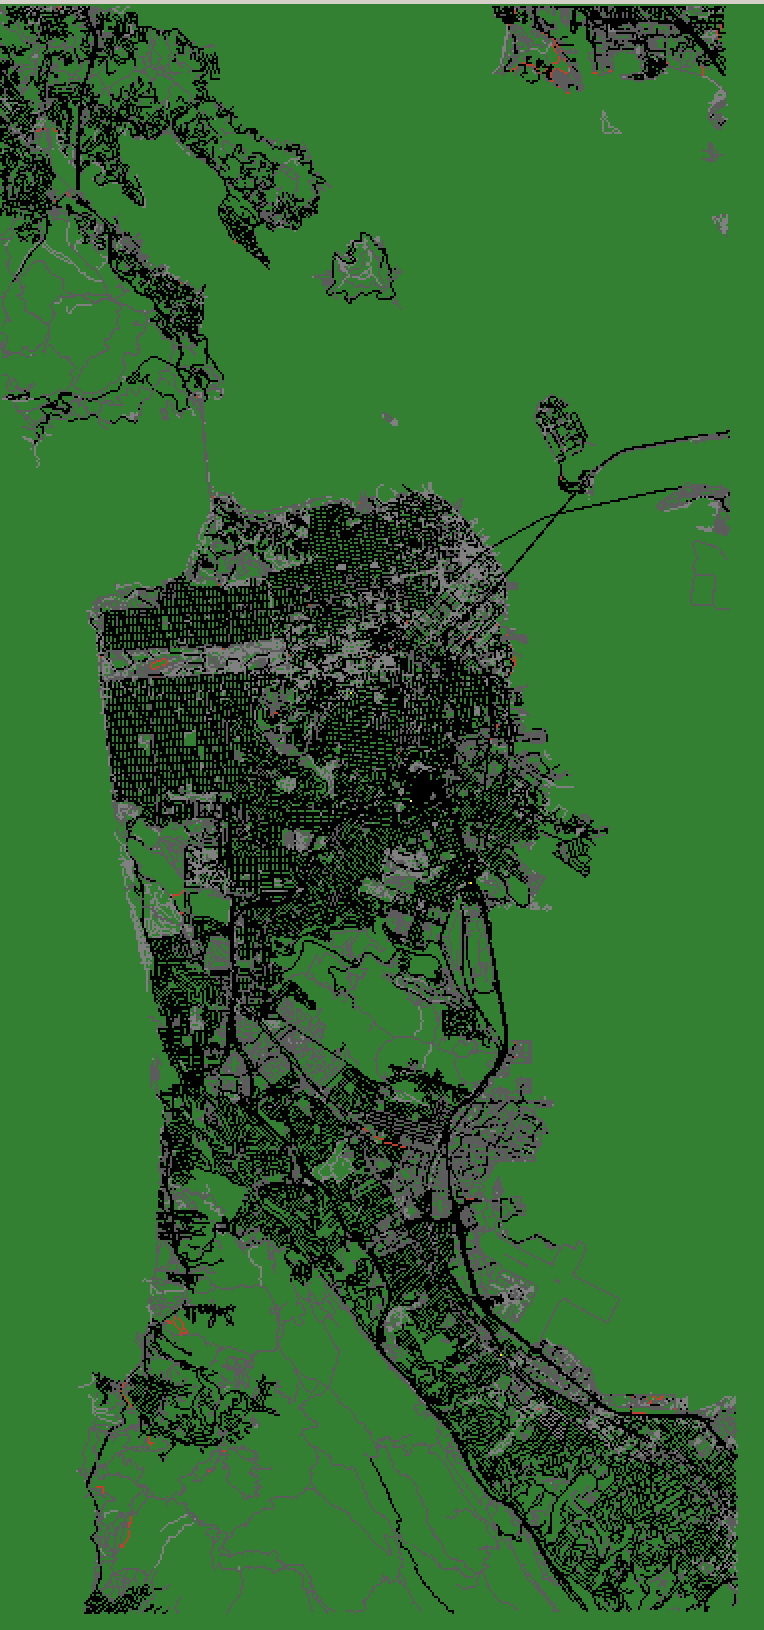
\includegraphics[width=0.40\linewidth]{data/ffss/sumo2.png}
    \caption{Sumo Map: San Francisco, California}
    \label{fig:Sumo2}
\end{figure}



In addition, we created a simulation for randomised traffic on the map, as seen in \ref{fig:Sumo2}. When connecting the API interface provided by the SUMO simulation with the GETACAR customer frontend and the virtual vehicles, future researchers can simulate the effects of the GETACAR ride-pooling platform on large road networks.

\begin{figure}[h]
    \centering
    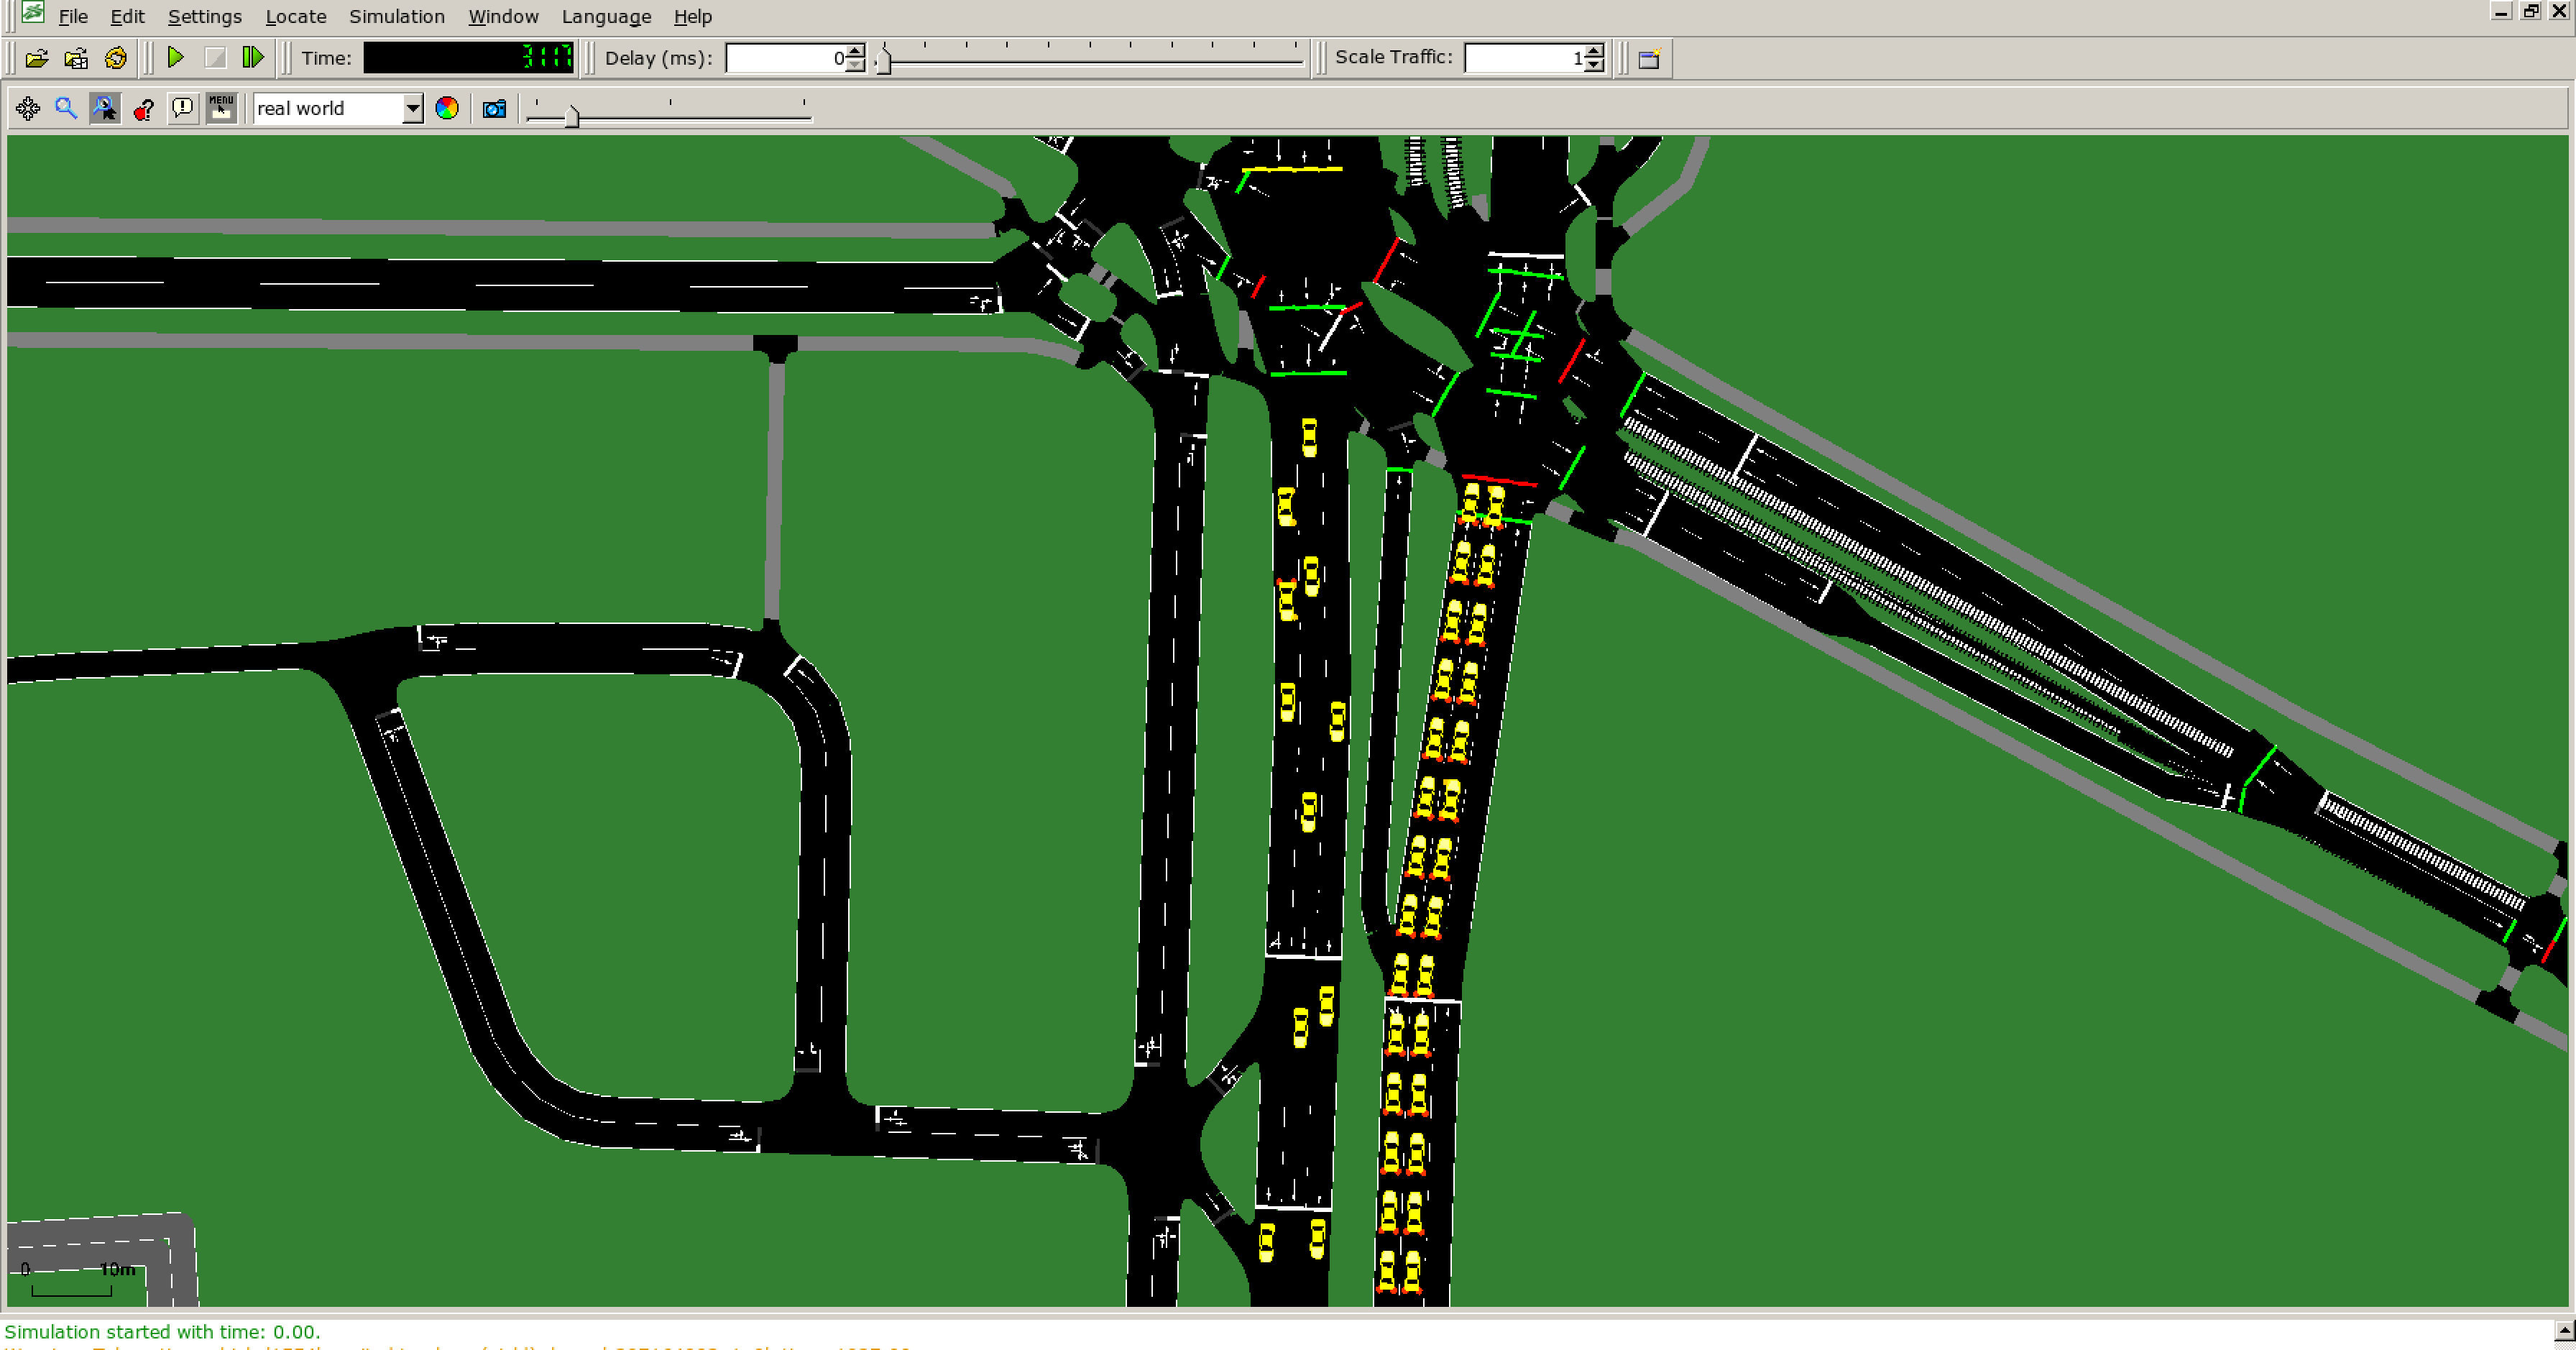
\includegraphics[width=0.90\linewidth]{data/ffss/sumo1.png}
    \caption{Sumo Traffic Simulation}
    \label{fig:Sumo1}
\end{figure}






